\documentclass[12pt,a4paper,spanish]{article} 

\usepackage{graphicx} %option specific for pdfLatex compilation
\usepackage{makeidx}
\usepackage{lscape}

\usepackage[spanish]{babel}
\usepackage[utf8]{inputenc} 
\usepackage{indentfirst}
\usepackage[margin=2cm]{geometry}

\author{\textbf{Grupo 2}\\Martín Buchwald\\Ezequiel Genender\\Andrés Lorek\\Luciano Sorrentino\\Jennifer Woites}
\title{75.43 Introducción a los Sistemas Distribuidos\\
	\textbf{Trabajo Práctico Grupal}\\
	Facultad de Ingeniería, Universidad de Buenos Aires
	\date{Cuatrimestre I, 2014}
}

\begin{document}
\maketitle
\thispagestyle{empty}
\newpage
\tableofcontents
\newpage

\section{Subnetting}
\subsection{Asignación de direcciones IP a las redes}
\begin{tabular}{|c|c|c|c|c|c|}
	\hline
	Subnet & Nombre & Hosts & Direcciones & Dirección & Máscara\\
	\hline
	A & Aguila & 125 & 128 & 201.158.15.0 & 255.255.255.128 \\
	\hline
	B & Buitre & 17 & 32 & 20.86.15.0 & 255.255.255.224 \\
	\hline
	C & Cuervo & 12 & 16 & 10.31.25.128 & 255.255.255.240 \\
	\hline
	D & Dodo & 223 & 256 & 20.64.73.0 & 255.255.255.0 \\
	\hline
	E & Espatula & 69 & 128 & 10.31.25.0 & 255.255.255.128 \\
	\hline
	F & Faisan & 19 & 32 & 20.86.15.32 & 255.255.255.224 \\
	\hline
	G & Golondrina & 2 & 4 & 10.31.25.152 & 255.255.255.252 \\
	\hline
	H & Hornero & 2 & 4 & 10.31.25.156 & 255.255.255.252 \\
	\hline
	I & Ibis & 10 PPP & & &\\
	\hline
	I1 &Ibis1 & 2 & 4 & 151.40.3.192 & 255.255.255.252 \\
	\hline
	I2 & Ibis2 & 2 & 4 & 151.40.3.196 & 255.255.255.252 \\ 
	\hline
	I3 & Ibis3 & 2 & 4 & 151.40.3.200 & 255.255.255.252 \\
	\hline
	I4 & Ibis4 & 2 & 4 & 151.40.3.204 & 255.255.255.252 \\
	\hline
	I5 & Ibis5 & 2 & 4 & 151.40.3.208 & 255.255.255.252 \\	
	\hline
	I6 &Ibis6 & 2 & 4 & 151.40.3.212 & 255.255.255.252 \\
	\hline
	I7 & Ibis7& 2 & 4 & 151.40.3.216 & 255.255.255.252 \\
	\hline
	I8 & Ibis8& 2 & 4 & 151.40.3.220 & 255.255.255.252 \\
	\hline
	I9 &Ibis9 & 2 & 4 & 151.40.3.224 & 255.255.255.252 \\
	\hline
	I10 &Ibis10 & 2 & 4 & 151.40.3.228 & 255.255.255.252 \\
	\hline
	J & Jilguero & 43 & 64 & 20.86.15.64 & 255.255.255.192 \\
	\hline
	K & Kiwi & 6 & 8 & 10.31.25.144 & 255.255.255.248 \\
	\hline
	L & Lechuza & 240 & 256 & 20.26.29.0 & 255.255.255.0 \\
	\hline
	M1 & Mero1 & 68 & 128 & 20.86.15.128 & 255.255.255.128 \\
	\hline
	M2 & Mero2 & 18 & 32 & 10.31.25.160 & 255.255.255.224 \\
	\hline
	N privada & Negron & 2 & 4 & 10.31.25.160 & 255.255.255.252 \\
	\hline
	O privada & Ortega & 2 & 4 & 10.31.25.164 & 255.255.255.252 \\
	\hline
	P privada & Paloma & 2 & 4 & 10.31.25.168 & 255.255.255.252 \\
	\hline
	Q1 Publica & Quebrantahuesos1 & 2 & 4 & 150.38.27.0 & 255.255.255.252 \\
	\hline
	Q2 Publica & Quebrantahuesos2 & 2 & 4 & 150.38.27.4 & 255.255.255.252 \\
	\hline
	Q3 Publica & Quebrantahuesos3 & 2 & 4 & 150.38.27.8 & 255.255.255.252 \\
	\hline
\end{tabular}



\subsubsection{Asignación IP a routers, servers, hosts}

\begin{tabular}{|c|c|c|c|c|}
	\hline
	Subred & Dispositivo & Interfaz & Dirección & Máscara\\
	\hline
	\hline
	A &  &  &  & \\
	\hline
	  & WebServer & & 201.158.15.1 & 255.255.255.128 \\
	\hline
	  & Host A & & 201.158.15.2 & 255.255.255.128 \\
	\hline
	  & R4 & e0/0 & 201.158.15.3 & 255.255.255.128 \\
	\hline
	  & R5 & e0/0 & 201.158.15.4 & 255.255.255.128 \\
	\hline
	  & R2 & e0/0 & 201.158.15.5 & 255.255.255.128 \\
	\hline
	  & R3 & e0/2 & 201.158.15.6 & 255.255.255.128 \\
	\hline
	  & Virtual A & & 201.158.15.7 & 255.255.255.128 \\
	\hline
	\hline
	B & & & & \\
	\hline
	  & R1 & e0/0 & 20.86.15.1 & 255.255.255.224 \\
	\hline
	  & R3 & e0/0 & 20.86.15.2 & 255.255.255.224 \\
	\hline
	\hline
	C & & & & \\
	\hline
	  & R1 & e0/1 & 10.31.25.129 & 255.255.255.240 \\
	\hline
  	  & R3 & e0/1 & 10.31.25.130 & 255.255.255.240 \\
	\hline
	\hline
	D & & & & \\
	\hline
	  & R5 & e0/1 & 20.64.73.1 & 255.255.255.0 \\
	\hline
	  & R4 & e0/1 & 20.64.73.2 & 255.255.255.0 \\
	\hline
	  & DNS-ROOT & & 20.64.73.3 & 255.255.255.0 \\
	\hline
	  & R8 & e0/0 & 20.64.73.4 & 255.255.255.0 \\
	\hline
	  & Virtual D & & 20.64.73.5 & 255.255.255.0 \\
	\hline
	\hline
	E & & & & \\
	\hline
	  & FTP-Server & & 10.31.25.1 & 255.255.255.128 \\
	\hline
	  & R12 & e0/0 & 10.31.25.2 & 255.255.255.128 \\
	\hline
	  & DNS1 & & 10.31.25.3 & 255.255.255.128 \\
	\hline
	  & R15 & e0/2 & 10.31.25.4 & 255.255.255.128 \\
	\hline
	  & R13 & e0/1 & 10.31.25.5 & 255.255.255.128 \\
	\hline
	\hline
	F & & & & \\
	\hline
	  & R13 & e0/0 & 20.86.15.33 & 255.255.255.224 \\
	\hline
	  & Host C & & 20.86.15.34 & 255.255.255.224 \\
	\hline
	  & R14 & e0/1 & 20.86.15.35 & 255.255.255.224 \\
	\hline
	\hline
	G & & & & \\
	\hline
	  & R10 & e1/2 & 10.31.25.153 & 255.255.255.252 \\
	\hline
	  & R13 & e0/2 & 10.31.25.154 & 255.255.255.252 \\
	\hline
	\hline
	H & & & & \\
	\hline
	  & R8 & e0/1 & 10.31.25.157 & 255.255.255.252 \\
	\hline
	  & R7 & e1/1 & 10.31.25.158 & 255.255.255.252 \\
	\hline
	\hline
	I1 & & & & \\
	\hline
	  & R2 & s1/0.1 & 151.40.3.193 & 255.255.255.252 \\
	\hline
	  & R17 & s1/0.1 & 151.40.3.194 & 255.255.255.252 \\
	\hline
	\hline
	I2 & & & & \\
	\hline
	  & R2 & s1/0.2 & 151.40.3.197 & 255.255.255.252 \\
	\hline
	  & R16 & s1/0.1 & 151.40.3.198 & 255.255.255.252 \\
	\hline
	\hline
	I3 & & & & \\
	\hline
	  & R2 & s1/0.3 & 151.40.3.201 & 255.255.255.252 \\
	\hline
	  & R9 & s1/0.1 & 151.40.3.202 & 255.255.255.252 \\
	\hline
\end{tabular}
\newpage
\begin{tabular}{|c|c|c|c|c|}
	\hline
	Subred & Dispositivo & Interfaz & Dirección & Máscara\\
	\hline
	\hline
	I4 & & & & \\
	\hline
	  & R2 & s1/0.4 & 151.40.3.205 & 255.255.255.252 \\
	\hline
	  & R6 & s1/0.1 & 151.40.3.206 & 255.255.255.252 \\
	\hline
	\hline
	I5 & & & & \\
	\hline
	  & R17 & s1/0.2 & 151.40.3.209 & 255.255.255.252 \\
	\hline
	  & R16 & s1/0.2 & 151.40.3.210 & 255.255.255.252 \\
	\hline
	\hline
	I6 & & & & \\
	\hline
	  & R17 & s1/0.3 & 151.40.3.213 & 255.255.255.252 \\
	\hline
	  & R9 & s1/0.2 & 151.40.3.214 & 255.255.255.252 \\
	\hline
	\hline
	I7 & & & & \\
	\hline
	  & R17 & s1/0.4 & 151.40.3.217 & 255.255.255.252 \\
	\hline
	  & R6 & s1/0.2 & 151.40.3.218 & 255.255.255.252 \\
	\hline
	\hline
	I8 & & & & \\
	\hline
	  & R16 & s1/0.3 & 151.40.3.221 & 255.255.255.252 \\
	\hline
	  & R9 & s1/0.3 & 151.40.3.222 & 255.255.255.252 \\
	\hline
	\hline
	I9 & & & & \\
	\hline
	  & R16 & s1/0.4 & 151.40.3.225 & 255.255.255.252 \\
	\hline
	  & R6 & s1/0.3 & 151.40.3.226 & 255.255.255.252 \\
	\hline
	\hline
	I10 & & & & \\
	\hline
	  & R9 & s1/0.4 & 151.40.3.229 & 255.255.255.252 \\
	\hline
	  & R6 & s1/0.4 & 151.40.3.230 & 255.255.255.252 \\
	\hline
	\hline
	J & & & & \\
	\hline
	  & R17 & e0/0 & 20.86.15.65 & 255.255.255.192 \\
	\hline
	  & R16 & e0/0 & 20.86.15.66 & 255.255.255.192 \\
	\hline
	  & R14 & e0/0 & 20.86.15.67 & 255.255.255.192 \\
	\hline
	  & R15 & e0/0 & 20.86.15.68 & 255.255.255.192 \\
	\hline
	\hline
	K & & & & \\
	\hline
	  & R15 & e0/1 & 10.31.25.145 & 255.255.255.248 \\
	\hline
	\hline
	L & & & & \\
	\hline
	  & R7 & e1/0 & 20.26.29.1 & 255.255.255.0 \\
	\hline
	  & R6 & e0/0 & 20.26.29.2 & 255.255.255.0 \\
	\hline
	  & R9 & e0/0 & 20.26.29.3 & 255.255.255.0 \\
	\hline
	  & Tel-Server & & 20.26.29.129 & 255.255.255.0 \\
	\hline
	\hline
	M1 & & & & \\
	\hline
	  & Host B & & 20.86.15.129 & 255.255.255.128 \\
	\hline
	  & Tel-Server & & 20.86.15.130 & 255.255.255.128 \\
	\hline
	  & R11 & e0/0 & 20.86.15.132 & 255.255.255.128 \\
	\hline
	  & R10 & e1/1 & 20.86.15.133 & 255.255.255.128 \\
	\hline
	\hline
	M2 & & & & \\
	\hline
	  & R10 & e1/0 & 10.31.25.193 & 255.255.255.224 \\
	\hline
	  & DNS2 & & 10.31.25.194 & 255.255.255.224 \\
	\hline
	\hline
	N & & & & \\
	\hline
	  & R8 & Tunnel10 & 10.31.25.161 & 255.255.255.252 \\
	\hline
	  & R11 & Tunnel10 & 10.31.25.162 & 255.255.255.252 \\
	\hline
\end{tabular}
\newpage
\begin{tabular}{|c|c|c|c|c|}
	\hline
	Subred & Dispositivo & Interfaz & Dirección & Máscara\\
	\hline
	\hline
	O & & & & \\
	\hline
	  & R8 & Tunnel20 & 10.31.25.165 & 255.255.255.252 \\
	\hline
	  & R12 & Tunnel20 & 10.31.25.166 & 255.255.255.252 \\
	\hline
	\hline
	P & & & & \\
	\hline
	  & R12 & Tunnel30 & 10.31.25.169 & 255.255.255.252 \\
	\hline
	  & R11 & Tunnel30 & 10.31.25.170 & 255.255.255.252 \\
	\hline
	Q1 & & & & \\
	\hline
	  & R8 & e0/2 & 150.38.27.1 & 255.255.255.252 \\
	\hline
	  & INTERNET & e1/0 & 150.38.27.2 & 255.255.255.252 \\
	\hline
	Q2 & & & & \\
	\hline
	  & R11 & e0/1 & 150.38.27.5 & 255.255.255.252 \\
	\hline
	  & INTERNET & e1/1 & 150.38.27.6 & 255.255.255.252 \\
	\hline
	Q3 & & & & \\
	\hline
	  & R12 & e0/1 & 150.38.27.9 & 255.255.255.252 \\
	\hline
	  & INTERNET & e1/2 & 150.38.27.10 & 255.255.255.252 \\
	\hline
\end{tabular}

\subsubsection{Asignación IP a routers en Frame Relay}

\begin{tabular}{|c|c|c|c|c|c|}
	\hline
	Subnet & Device & Interface & Address & Mask & DLCI \\
	\hline	
	I1 & R2 & s1/0.1 & 151.40.3.193 & 255.255.255.252 & 217 \\
	\hline
	   & R17 & s1/0.1 & 151.40.3.194 & 255.255.255.252 & 172 \\
	\hline
	I2 & R2 & s1/0.2 & 151.40.3.197 & 255.255.255.252 & 216 \\ 
	\hline
	   & R16 & s1/0.1 & 151.40.3.198 & 255.255.255.252 & 162 \\ 
	\hline
	I3 & R2 & s1/0.3 & 151.40.3.201 & 255.255.255.252 & 209 \\
	\hline
	   & R9 & s2/0.1 & 151.40.3.202 & 255.255.255.252 & 902 \\
	\hline
	I4 & R2 & s1/0.4 & 151.40.3.205 & 255.255.255.252 & 206 \\
	\hline
	   & R6 & s1/0.1 & 151.40.3.206 & 255.255.255.252 & 602 \\
	\hline
	I5 & R17 & s1/0.2  & 151.40.3.209 & 255.255.255.252 & 807 \\	
	\hline
	   & R16 & s1/0.2 & 151.40.3.210 & 255.255.255.252 & 708 \\	
	\hline
	I6 & R17 & s1/0.3 & 151.40.3.213 & 255.255.255.252 & 179 \\
	\hline
	   & R9 & s2/0.2 & 151.40.3.214 & 255.255.255.252 & 917 \\
	\hline
	I7 & R17 & s1/0.4 & 151.40.3.217 & 255.255.255.252 & 176 \\
	\hline
	   & R6 & s1/0.2 & 151.40.3.218 & 255.255.255.252 & 617 \\
	\hline
	I8 & R16 & s1/0.3 & 151.40.3.221 & 255.255.255.252 & 169 \\
	\hline
	   & R9 & s2/0.3 & 151.40.3.222 & 255.255.255.252 & 916 \\
	\hline
	I9 & R16 & s1/0.4 & 151.40.3.225 & 255.255.255.252 & 166 \\
	\hline
	   & R6 & s1/0.3 & 151.40.3.226 & 255.255.255.252 & 616 \\
	\hline
	I10 & R9 & s2/0.4 & 151.40.3.229 & 255.255.255.252 & 906 \\
	\hline
	    & R6 & s1/0.4 & 151.40.3.230 & 255.255.255.252 & 609 \\
	\hline
\end{tabular}


\subsection{Tablas de Ruteo de Córdoba}

\subsubsection{R1}
\begin{tabular}{|c|c|c|c|c|c|}
	\hline
	Red & Dirección de Red & Máscara & Sig. Salto & Dir. Sig. Salto & Métrica \\
	\hline
	& 0.0.0.0 & 0.0.0.0 & R3 & 20.86.15.2 & 1\\
	\hline
\end{tabular}


\subsubsection{R2}
\begin{tabular}{|c|c|c|c|c|c|}
	\hline
	Red & Dirección de Red & Máscara & Sig. Salto & Dir. Sig. Salto & Métrica \\
	\hline
	A & Directamente conectado & & & &\\
	\hline	
	B & 20.86.15.0 & 255.255.255.224 & R3 & 201.158.15.6 & 1\\
	\hline
	C & 10.31.25.128 & 255.255.255.240 & R3 & 201.158.15.6 & 1\\
	\hline
	D & 20.64.73.0 & 255.255.255.0 & Virtual-A &  201.158.15.7 & 1\\
	\hline
	E & 10.31.25.0 & 255.255.255.128 & R17 & 151.40.3.194 & 1\\
	\hline
	F & 20.86.15.32 & 255.255.255.224 & R17 & 151.40.3.194 & 1\\
	\hline
	G & 10.31.25.152 & 255.255.255.252 & R17 & 151.40.3.194 & 1\\
	\hline
	H & 10.31.25.156 & 255.255.255.252 & Virtual-A &  201.158.15.7 & 1\\
	\hline
	I &  & & & &\\
	I1 & Directamente conectado &&&& \\
	I2 & Directamente conectado &&&& \\
	I3 & Directamente conectado &&&& \\
	I4 & Directamente conectado &&&& \\
	I5 & 151.40.3.208 & 255.255.255.252 & R17 & 151.40.3.194 & 1 \\
	   &              &                 & R16 & 151.40.3.198 & 10 \\
 	I6 & 151.40.3.212 & 255.255.255.252 & R17 & 151.40.3.194 & 1 \\
 	   &              &                 & R9 & 151.40.3.202 & 10 \\
 	I7 & 151.40.3.216 & 255.255.255.252 & R17 & 151.40.3.194 & 1 \\
 	   &              &                 & R6 & 151.40.3.206 & 10 \\
 	I8 & 151.40.3.220 & 255.255.255.252 & R16 & 151.40.3.198 & 1 \\
 	   &              &                 & R9 & 151.40.3.202 & 10 \\
 	I9 & 151.40.3.224 & 255.255.255.252 & R16 & 151.40.3.198 & 1 \\
 	   &              &                 & R6 & 151.40.3.206 & 10 \\
 	I10 & 151.40.3.228 & 255.255.255.252 & R9 & 151.40.3.202 & 1 \\
 	   &              &                 & R6 & 151.40.3.206 & 10 \\
	\hline
	J & 20.86.15.64 & 255.255.255.192 & R17 & 151.40.3.194 & 1\\
 	\hline
	K & 10.31.25.144 & 255.255.255.248 & R17 & 151.40.3.194 & 1\\
 	\hline
	L & 20.26.29.0 & 255.255.255.0 & R9 & 151.40.3.202 & 1\\
	  &            &               & R6 & 151.40.3.206 & 10\\
	\hline
	M1 & 20.86.15.128 & 255.255.255.128 & Virtual-A &  201.158.15.7 & 1\\
	\hline
	M2 & 10.31.25.192 & 255.255.255.224 & Virtual-A &  201.158.15.7 & 1\\
	\hline
	N & 10.31.25.160 & 255.255.255.252 & Virtual-A & 201.158.15.7 & 1\\
	\hline
	O & 10.31.25.164 & 255.255.255.252 & Virtual-A & 201.158.15.7 & 1\\
	\hline
	P & 10.31.25.168 & 255.255.255.252 & Virtual-A & 201.158.15.7 & 1\\
	\hline
\end{tabular}


\subsubsection{R3}
\begin{tabular}{|c|c|c|c|c|c|}
	\hline
	Red & Dirección de Red & Máscara & Sig. Salto & Dir. Sig. Salto & Métrica \\
	\hline
	A & Directamente conectado & & & &\\
	\hline	
	B & Directamente conectado & & & &\\
	\hline
	C & Directamente conectado & & & &\\
	\hline
	D & 20.64.73.0 & 255.255.255.0 & Virtual-A & 201.158.15.7 & 1\\
	\hline
	E & 10.31.25.0 & 255.255.255.128 & R2 & 201.158.15.5 & 1\\
	\hline
	F & 20.86.15.32 & 255.255.255.224 & R2 & 201.158.15.5 & 1\\
	\hline
	G & 10.31.25.152 & 255.255.255.252 & R2 & 201.158.15.5 & 1\\
	\hline
	H & 10.31.25.156 & 255.255.255.252 & Virtual-A & 201.158.15.7 & 1\\
	\hline
	I &  & & & &\\
	I1 & 151.40.3.192 & 255.255.255.252 & R2 & 201.158.15.5  & 1 \\
	I2 & 151.40.3.196 & 255.255.255.252 & R2 & 201.158.15.5 & 1 \\
 	I3 & 151.40.3.200 & 255.255.255.252 & R2 & 201.158.15.5 & 1 \\
 	I4 & 151.40.3.204 & 255.255.255.252 & R2 & 201.158.15.5 & 1 \\
 	I5 & 151.40.3.208 & 255.255.255.252 & R2 & 201.158.15.5 & 1 \\
 	I6 & 151.40.3.212 & 255.255.255.252 & R2 & 201.158.15.5 & 1 \\
 	I7 & 151.40.3.216 & 255.255.255.252 & R2 & 201.158.15.5 & 1 \\
 	I8 & 151.40.3.220 & 255.255.255.252 & R2 & 201.158.15.5 & 1 \\
 	I9 & 151.40.3.224 & 255.255.255.252 & R2 & 201.158.15.5 & 1 \\
 	I10 & 151.40.3.228 & 255.255.255.252 & R2 & 201.158.15.5 & 1 \\
	\hline
	J & 20.86.15.64 & 255.255.255.192 & R2 & 201.158.15.5 & 1\\
 	\hline
	K & 10.31.25.144 & 255.255.255.248 & R2 & 201.158.15.5 & 1\\
 	\hline
	L & 20.26.29.0 & 255.255.255.0 & R2 & 201.158.15.5 & 1\\
	  &            &               & Virtual-A & 201.158.15.7 & 100\\
	\hline
	M1 & 20.86.15.128 & 255.255.255.128 & Virtual-A & 201.158.15.7 & 1\\
	\hline
	M2 & 10.31.25.192 & 255.255.255.224 & Virtual-A & 201.158.15.7 & 1\\
	\hline
	N & 10.31.25.160 & 255.255.255.252 & Virtual-A & 201.158.15.7 & 1\\
	\hline
	O & 10.31.25.164 & 255.255.255.252 & Virtual-A & 201.158.15.7 & 1\\
	\hline
	P & 10.31.25.168 & 255.255.255.252 & R2 & 201.158.15.5 & 1\\
	\hline
\end{tabular}

\subsubsection{R4 y R5 (routers VRRP)}
\begin{tabular}{|c|c|c|c|c|c|}
	\hline
	Red & Dirección de Red & Máscara & Sig. Salto & Dir. Sig. Salto & Métrica \\
	\hline
	A & Directamente conectado &&&&\\
	\hline	
	B & 20.86.15.0 & 255.255.255.224 & R3 & 201.158.15.6 & 1\\
	\hline
	C & 10.31.25.128 & 255.255.255.240 & R3 & 201.158.15.6 & 1\\
	\hline
	D & Directamente conectado &&&&\\
	\hline
	E & 10.31.25.0 & 255.255.255.128 & R2 & 201.158.15.5 & 1\\
	  &            &                 & R8  & 20.64.73.4  & 100\\
	\hline
	F & 20.86.15.32 & 255.255.255.224 &  R2 & 201.158.15.5& 1\\
	  &            &                 & R8  & 20.64.73.4  & 100\\
	\hline
	G & 10.31.25.152 & 255.255.255.252 &  R2 & 201.158.15.5 & 1\\
	  &            &                 & R8  & 20.64.73.4  & 100\\
	\hline
	H & 10.31.25.156 & 255.255.255.252 & R8 & 20.64.73.4 & 1\\
	\hline
	I &  & & & &\\
	I1 & 151.40.3.192 & 255.255.255.252 & R2 & 201.158.15.5 & 1 \\
	I2 & 151.40.3.196 & 255.255.255.252 & R2 & 201.158.15.5 & 1 \\
 	I3 & 151.40.3.200 & 255.255.255.252 & R2 & 201.158.15.5 & 1 \\
 	I4 & 151.40.3.204 & 255.255.255.252 & R2 & 201.158.15.5 & 1 \\
 	I5 & 151.40.3.208 & 255.255.255.252 & R2 & 201.158.15.5 & 1 \\
 	I6 & 151.40.3.212 & 255.255.255.252 & R2 & 201.158.15.5 & 1 \\
 	I7 & 151.40.3.216 & 255.255.255.252 & R2 & 201.158.15.5 & 1 \\
 	I8 & 151.40.3.220 & 255.255.255.252 & R2 & 201.158.15.5 & 1 \\
 	I9 & 151.40.3.224 & 255.255.255.252 & R2 & 201.158.15.5 & 1 \\
 	I10 & 151.40.3.228 & 255.255.255.252 & R2 & 201.158.15.5 & 1 \\
	\hline
	J & 20.86.15.64 & 255.255.255.192 & R2 & 201.158.15.5 & 1\\
	  &            &                 & R8  & 20.64.73.4  & 100\\
 	\hline
	K & 10.31.25.144 & 255.255.255.248 & R2 & 201.158.15.5 & 1\\
	  &            &                 & R8  & 20.64.73.4  & 100\\
 	\hline
	L & 20.26.29.0 & 255.255.255.0 & R8 & 20.64.73.4 & 1\\
	\hline
	M1 & 20.86.15.128 & 255.255.255.128 & R8 & 20.64.73.4 & 1\\
	\hline
	M2 & 10.31.25.192 & 255.255.255.224 & R8 & 20.64.73.4 & 1\\
	\hline
	N & 10.31.25.160 & 255.255.255.252 & R8 & 20.64.73.4& 1\\
	\hline
	O & 10.31.25.164 & 255.255.255.252 & R8 & 20.64.73.4 & 1\\
	\hline
	P & 10.31.25.168 & 255.255.255.252 & R8 & 20.64.73.4 & 1\\
	\hline
\end{tabular}


\subsubsection{R8}
\begin{tabular}{|c|c|c|c|c|c|}
	\hline
	Red & Dirección de Red & Máscara & Sig. Salto & Dir. Sig. Salto & Métrica \\
	\hline
	A & 201.158.15.0  & 255.255.255.128 & Virtual-D & 20.64.73.5 & 1\\
	\hline	
	B & 20.86.15.0 & 255.255.255.224 & Virtual-D & 20.64.73.5 & 1\\
	\hline
	C & 10.31.25.128 & 255.255.255.240 & Virtual-D & 20.64.73.5 & 1\\
	\hline
	D & Directamente conectado &&&&\\
	\hline
	E & 10.31.25.0 & 255.255.255.128 & R12 & 10.31.25.166 & 1\\
	\hline
	F & 20.86.15.32 & 255.255.255.224 &R12 & 10.31.25.166 & 1\\
	\hline
	G & 10.31.25.152 & 255.255.255.252 & R12 & 10.31.25.166 & 1\\
	\hline
	H & Directamente conectado &&&&\\
	\hline
	I &  & & & &\\
	I1 & 151.40.3.192 & 255.255.255.252 & Virtual-D & 20.64.73.5 & 1 \\
	I2 & 151.40.3.196 & 255.255.255.252 & Virtual-D & 20.64.73.5 & 1 \\
 	I3 & 151.40.3.200 & 255.255.255.252 & Virtual-D & 20.64.73.5 & 1 \\
 	I4 & 151.40.3.204 & 255.255.255.252 & Virtual-D & 20.64.73.5 & 1 \\
 	I5 & 151.40.3.208 & 255.255.255.252 & Virtual-D & 20.64.73.5 & 1 \\
 	I6 & 151.40.3.212 & 255.255.255.252 & Virtual-D & 20.64.73.5 & 1 \\
 	I7 & 151.40.3.216 & 255.255.255.252 & Virtual-D & 20.64.73.5 & 1 \\
 	I8 & 151.40.3.220 & 255.255.255.252 & Virtual-D & 20.64.73.5 & 1 \\
 	I9 & 151.40.3.224 & 255.255.255.252 & Virtual-D & 20.64.73.5 & 1 \\
 	I10 & 151.40.3.228 & 255.255.255.252 & Virtual-D & 20.64.73.5 & 1 \\
	\hline
	J & 20.86.15.64 & 255.255.255.192 & R12 & 10.31.25.166 & 1\\
 	\hline
	K & 10.31.25.144 & 255.255.255.248 & R12 & 10.31.25.166 & 1\\
 	\hline
	L & 20.26.29.0 & 255.255.255.0 & R7 & 10.31.25.158 & 1\\
	\hline
	M1 & 20.86.15.128 & 255.255.255.128 & R11 & 10.31.25.162 & 1\\
	\hline
	M2 & 10.31.25.192 & 255.255.255.224 & R11 & 10.31.25.162 & 1\\
	\hline
	N & Directamente conectada &&&& \\
	\hline
	O & Directamente conectada &&&& \\
	\hline
	P & 10.31.25.168 & 255.255.255.252 & R12 & 10.31.25.166 & 1\\
	\hline
\end{tabular}


\subsection{Tablas de Ruteo de Calamuchita}
\subsubsection{R6}
\begin{tabular}{|c|c|c|c|c|c|}
	\hline
	Red & Dirección de Red & Máscara & Sig. Salto & Dir. Sig. Salto & Métrica \\
	\hline
	A & 201.158.15.0  & 255.255.255.128 & R2 & 151.40.3.205 & 1\\
	  &               &                 & R9 & 20.26.29.3& 10\\
	\hline	
	B & 20.86.15.0 & 255.255.255.224 & R2 & 151.40.3.205 & 1\\
	  &               &                 & R9 & 20.26.29.3& 10\\
	\hline
	C & 10.31.25.128 & 255.255.255.240 & R2 & 151.40.3.205 & 1\\
	  &               &                 & R9 & 20.26.29.3& 10\\
	\hline
	D & 20.64.73.0 & 255.255.255.0 & R7 & 20.26.29.1 & 1\\
	  &            &               & R2 & 151.40.3.205 & 10\\
	\hline
	E & 10.31.25.0 & 255.255.255.128 & R17 & 151.40.3.217 & 1\\
		  &               &                 & R9 & 20.26.29.3& 10\\
	\hline
	F & 20.86.15.32 & 255.255.255.224 & R17 & 151.40.3.217 & 1\\
		  &               &                 & R9 & 20.26.29.3& 10\\
	\hline
	G & 10.31.25.152 & 255.255.255.252 & R17 & 151.40.3.217 & 1\\
		  &               &                 & R9 & 20.26.29.3& 10\\
	\hline
	H & 10.31.25.156 & 255.255.255.252 & R7 & 20.26.29.1 & 1\\
	\hline
	I &  & & & &\\
	I1 & 151.40.3.192 & 255.255.255.252 &  R2 & 151.40.3.205 & 1 \\
	   &              &                 &  R17 & 151.40.3.217 & 10 \\
	I2 & 151.40.3.196 & 255.255.255.252 &  R2 & 151.40.3.205 & 1 \\
	   &              &                 &  R16 & 151.40.3.225 & 10 \\	
 	I3 & 151.40.3.200 & 255.255.255.252 &  R2 & 151.40.3.205 & 1 \\
 		   &              &                 &  R9 & 151.40.3.229 & 10 \\
 	I4 & Directamente conectado &&&& \\
 	I5 & 151.40.3.208 & 255.255.255.252 & R17 & 151.40.3.217 & 1 \\
	   &              &                 &  R16 & 151.40.3.225 & 10 \\
 	I6 & 151.40.3.212 & 255.255.255.252 & R17 & 151.40.3.217 & 1 \\
	   &              &                 &  R9 & 151.40.3.229 & 10 \\
 	I7 & Directamente conectado &&&& \\
 	I8 & 151.40.3.220 & 255.255.255.252 & R9 & 151.40.3.229 & 1 \\
 	   &              &                 &  R16 & 151.40.3.225 & 10 \\
 	I9 & Directamente conectado &&&& \\
 	I10 & Directamente conectado &&&& \\
 	\hline
	J & 20.86.15.64 & 255.255.255.192 & R17 & 151.40.3.217 & 1\\
 	\hline
	K & 10.31.25.144 & 255.255.255.248 & R17 & 151.40.3.217 & 1\\
 	\hline
	L & Directamente conectado &&&&\\
	\hline
	M1 & 20.86.15.128 & 255.255.255.128 & R7 & 20.26.29.1 & 1\\
	\hline
	M2 & 10.31.25.192 & 255.255.255.224 & R7 & 20.26.29.1 & 1\\
	\hline
	N & 10.31.25.160 & 255.255.255.252 & R7 & 20.26.29.1& 1\\
	\hline
	O & 10.31.25.164 & 255.255.255.252 & R7 & 20.26.29.1 & 1\\
	\hline
	P & 10.31.25.168 & 255.255.255.252 & R7 & 20.26.29.1 & 1\\
	\hline
\end{tabular}


\subsubsection{R7}
\begin{tabular}{|c|c|c|c|c|c|}
	\hline
	Red & Dirección de Red & Máscara & Sig. Salto & Dir. Sig. Salto & Métrica \\
	\hline
	A & 201.158.15.0  & 255.255.255.128 & R6 & 20.26.29.2 & 1\\
	 &                &                 & R8 & 10.31.25.157 & 100\\
	\hline	
	B & 20.86.15.0 & 255.255.255.224 & R6 & 20.26.29.2 & 1\\
	 &                &                 & R8 & 10.31.25.157 & 100\\
	\hline
	C & 10.31.25.128 & 255.255.255.240 & R6 & 20.26.29.2 & 1\\
	 &                &                 & R8 & 10.31.25.157 & 100\\
	\hline
	D & 20.64.73.0 & 255.255.255.0 & R8 & 10.31.25.157 & 1\\
	 &                &                 & R6 & 20.26.29.2 & 10\\
	\hline
	E & 10.31.25.0 & 255.255.255.128 & R6 & 20.26.29.2 & 1\\
	\hline
	F & 20.86.15.32 & 255.255.255.224 & R6 & 20.26.29.2 & 1\\
	\hline
	G & 10.31.25.152 & 255.255.255.252 & R6 & 20.26.29.2 & 1\\
	\hline
	H & Directamente conectado &&&&\\
	\hline
	I &  & & & &\\
	I1 & 151.40.3.192 & 255.255.255.252 & R6 & 20.26.29.2 & 1 \\
	I2 & 151.40.3.196 & 255.255.255.252 & R6 & 20.26.29.2 & 1 \\
 	I3 & 151.40.3.200 & 255.255.255.252 & R6 & 20.26.29.2 & 1 \\
 	I4 & 151.40.3.204 & 255.255.255.252 & R6 & 20.26.29.2 & 1 \\
 	I5 & 151.40.3.208 & 255.255.255.252 & R6 & 20.26.29.2 & 1 \\
 	I6 & 151.40.3.212 & 255.255.255.252 & R6 & 20.26.29.2 & 1 \\
 	I7 & 151.40.3.216 & 255.255.255.252 & R6 & 20.26.29.2 & 1 \\
 	I8 & 151.40.3.220 & 255.255.255.252 & R6 & 20.26.29.2 & 1 \\
 	I9 & 151.40.3.224 & 255.255.255.252 & R6 & 20.26.29.2 & 1 \\
 	I10 & 151.40.3.228 & 255.255.255.252 & R6 & 20.26.29.2 & 1 \\
	\hline
	J & 20.86.15.64 & 255.255.255.192 & R6 & 20.26.29.2 & 1\\
 	\hline
	K & 10.31.25.144 & 255.255.255.248 & R6 & 20.26.29.2 & 1\\
 	\hline
	L & Directamente conectada &&&&\\
	\hline
	M1 & 20.86.15.128 & 255.255.255.128 & R8 & 10.31.25.157 & 1\\
	\hline
	M2 & 10.31.25.192 & 255.255.255.224 & R8 & 10.31.25.157 & 1\\
	\hline
	N & 10.31.25.160 & 255.255.255.252 & R8 & 10.31.25.157 & 1\\
	\hline
	O & 10.31.25.164 & 255.255.255.252 & R8 & 10.31.25.157 & 1\\
	\hline
	P & 10.31.25.168 & 255.255.255.252 & R8 & 10.31.25.157 & 1\\
	\hline
\end{tabular}

\subsubsection{R9}
\begin{tabular}{|c|c|c|c|c|c|}
	\hline
	Red & Dirección de Red & Máscara & Sig. Salto & Dir. Sig. Salto & Métrica \\
	\hline
	A & 201.158.15.0  & 255.255.255.128 & R2 & 151.40.3.201 & 1\\
	\hline	
	B & 20.86.15.0 & 255.255.255.224 & R2 & 151.40.3.201 & 1\\
	\hline
	C & 10.31.25.128 & 255.255.255.240 & R2 & 151.40.3.201 & 1\\
	\hline
	D & 20.64.73.0 & 255.255.255.0 & R2 & 151.40.3.201 & 1\\
	\hline
	E & 10.31.25.0 & 255.255.255.128 & R17 & 151.40.3.213 & 1\\
      &            &                 & R16 & 151.40.3.221& 10\\
	\hline
	F & 20.86.15.32 & 255.255.255.224 & R17 & 151.40.3.213 & 1\\
      &            &                 & R16 & 151.40.3.221& 10\\
	\hline
	G & 10.31.25.152 & 255.255.255.252 & R17 & 151.40.3.213 & 1\\
      &            &                 & R16 & 151.40.3.221& 10\\
	\hline
	H & 10.31.25.156 & 255.255.255.252 & R7 & 20.26.29.1 & 1\\
	\hline
	I &  & & & &\\
	I1 & 151.40.3.192 & 255.255.255.252 & R2 & 151.40.3.201 & 1 \\
       &              &                 & R17 & 151.40.3.213 & 10\\	
	I2 & 151.40.3.196 & 255.255.255.252 & R2 & 151.40.3.201 & 1 \\
       &              &                 & R16 & 151.40.3.221 & 10\\	
 	I3 & Directamente conectada &&&& \\
 	I4 & 151.40.3.204 & 255.255.255.252 & R2 & 151.40.3.201 & 1 \\
       &              &                 & R6 & 151.40.3.230 & 10\\	
 	I5 & 151.40.3.208 & 255.255.255.252 & R17 & 151.40.3.213 & 1 \\
       &              &                 & R16 & 151.40.3.221 & 10\\	
 	I6 & Directamente conectada &&&& \\
 	I7 & 151.40.3.216 & 255.255.255.252 & R17 & 151.40.3.213 & 1 \\
       &              &                 & R6 & 151.40.3.230 & 10\\	
 	I8 & Directamente conectada &&&& \\
 	I9 & 151.40.3.224 & 255.255.255.252 & R6 & 20.86.15.2 & 1 \\
       &              &                 & R16 & 151.40.3.221 & 10\\	
 	I10 & Directamente conectada &&&& \\
	\hline
	J & 20.86.15.64 & 255.255.255.192 & R17 & 151.40.3.213 & 1\\
	       &              &                 & R16 & 151.40.3.221 & 10\\	
 	\hline
	K & 10.31.25.144 & 255.255.255.248 & R17 & 151.40.3.213 & 1\\
	       &              &                 & R16 & 151.40.3.221 & 10\\	
 	\hline
	L & Directamente conectada &&&&\\
	\hline
	M1 & 20.86.15.128 & 255.255.255.128 & R7 & 20.26.29.1 & 1\\
	\hline
	M2 & 10.31.25.192 & 255.255.255.224 & R7 & 20.26.29.1 & 1\\
	\hline
	N & 10.31.25.160 & 255.255.255.252 & R7 & 20.26.29.1 & 1\\
	\hline
	O & 10.31.25.164 & 255.255.255.252 & R7 & 20.26.29.1 & 1\\
	\hline
	P & 10.31.25.168 & 255.255.255.252 & R7 & 20.26.29.1 & 1\\
	\hline
\end{tabular}

\subsubsection{R10}
\begin{tabular}{|c|c|c|c|c|c|}
	\hline
	Red & Dirección de Red & Máscara & Sig. Salto & Dir. Sig. Salto & Métrica \\
	\hline
	A & 201.158.15.0  & 255.255.255.128 & R11 & 20.86.15.132 & 1\\
	\hline	
	B & 20.86.15.0 & 255.255.255.224 & R11 & 20.86.15.132 & 1\\
	\hline
	C & 10.31.25.128 & 255.255.255.240 & R11 & 20.86.15.132 & 1\\
	\hline
	D & 20.64.73.0 & 255.255.255.0 & R11 & 20.86.15.132 & 1\\
	\hline
	E & 10.31.25.0 & 255.255.255.128 & R13 & 10.31.25.154 & 1\\
	\hline
	F & 20.86.15.32 & 255.255.255.224 & R13 & 10.31.25.154 & 1\\
	\hline
	G & Directamente conectada &&&&\\
	\hline
	H & 10.31.25.156 & 255.255.255.252 & R11 & 20.86.15.132 & 1\\
	\hline
	I &  & & & &\\
	I1 & 151.40.3.192 & 255.255.255.252 & R13 & 10.31.25.154 & 1 \\
	I2 & 151.40.3.196 & 255.255.255.252 & R13 & 10.31.25.154 & 1 \\
 	I3 & 151.40.3.200 & 255.255.255.252 & R13 & 10.31.25.154 & 1 \\
 	I4 & 151.40.3.204 & 255.255.255.252 & R13 & 10.31.25.154 & 1 \\
 	I5 & 151.40.3.208 & 255.255.255.252 & R13 & 10.31.25.154 & 1 \\
 	I6 & 151.40.3.212 & 255.255.255.252 & R13 & 10.31.25.154 & 1 \\
 	I7 & 151.40.3.216 & 255.255.255.252 & R13 & 10.31.25.154 & 1 \\
 	I8 & 151.40.3.220 & 255.255.255.252 & R13 & 10.31.25.154 & 1 \\
 	I9 & 151.40.3.224 & 255.255.255.252 & R13 & 10.31.25.154 & 1 \\
 	I10 & 151.40.3.228 & 255.255.255.252 & R13 & 10.31.25.154 & 1 \\
	\hline
	J & 20.86.15.64 & 255.255.255.192 & R13 & 10.31.25.154 & 1\\
 	\hline
	K & 10.31.25.144 & 255.255.255.248 & R13 & 10.31.25.154 & 1\\
 	\hline
	L & 20.26.29.0 & 255.255.255.0 & R11 & 20.86.15.132 & 1\\
	\hline
	M1 & Directamente conectada &&&&\\
	\hline
	M2 & Directamente conectada &&&&\\
	\hline
	N & 10.31.25.160 & 255.255.255.252 & R11 & 20.86.15.132 & 1\\
	\hline
	O & 10.31.25.164 & 255.255.255.252 & R11 & 20.86.15.132 & 1\\
	\hline
	P & 10.31.25.168 & 255.255.255.252 & R11 & 20.86.15.132 & 1\\
	\hline
\end{tabular}


\subsubsection{R11}
\textbf{REVISAR POR REDES: A, B, C, D, E, H, J, K, L, O}\\
\begin{tabular}{|c|c|c|c|c|c|}
	\hline
	Red & Dirección de Red & Máscara & Sig. Salto & Dir. Sig. Salto & Métrica \\
	\hline
	A & 201.158.15.0  & 255.255.255.128 & R8 & 10.31.25.161 & 1\\
	\hline	
	B & 20.86.15.0 & 255.255.255.224 & R8 & 10.31.25.161 & 1\\
	\hline
	C & 10.31.25.128 & 255.255.255.240 & R8 & 10.31.25.161 & 1\\
	\hline
	D & 20.64.73.0 & 255.255.255.0 & R8 & 10.31.25.161 & 1\\
	\hline
	E & 10.31.25.0 & 255.255.255.128 & R12 & 10.31.25.169 & 1\\
	\hline
	F & 20.86.15.32 & 255.255.255.224 & R10 & 20.86.15.133 & 1\\
	\hline
	G & 10.31.25.152 & 255.255.255.252 & R10 & 20.86.15.133 & 1\\
	\hline
	H & 10.31.25.156 & 255.255.255.252 & R8 & 10.31.25.161 & 1\\
	\hline
	I &  & & & &\\
	I1 & 151.40.3.192 & 255.255.255.252 & R10 & 20.86.15.133 & 1 \\
	I2 & 151.40.3.196 & 255.255.255.252 & R10 & 20.86.15.133 & 1 \\
 	I3 & 151.40.3.200 & 255.255.255.252 & R10 & 20.86.15.133 & 1 \\
 	I4 & 151.40.3.204 & 255.255.255.252 & R10 & 20.86.15.133 & 1 \\
 	I5 & 151.40.3.208 & 255.255.255.252 & R10 & 20.86.15.133 & 1 \\
 	I6 & 151.40.3.212 & 255.255.255.252 & R10 & 20.86.15.133 & 1 \\
 	I7 & 151.40.3.216 & 255.255.255.252 & R10 & 20.86.15.133 & 1 \\
 	I8 & 151.40.3.220 & 255.255.255.252 & R10 & 20.86.15.133 & 1 \\
 	I9 & 151.40.3.224 & 255.255.255.252 & R10 & 20.86.15.133 & 1 \\
 	I10 & 151.40.3.228 & 255.255.255.252 & R10 & 20.86.15.133 & 1 \\
	\hline
	J & 20.86.15.64 & 255.255.255.192 & R12 & 10.31.25.169 & 1\\
 	\hline
	K & 10.31.25.144 & 255.255.255.248 & R12 & 10.31.25.169 & 1\\
 	\hline
	L & 20.26.29.0 & 255.255.255.0 & R8 & 10.31.25.161 & 1\\
	\hline
	M1 & Directamente conectada &&&&\\
	\hline
	M2 & 10.31.25.192 & 255.255.255.224 & R10 & 20.86.15.133 & 1\\
	\hline
	N & Directamente conectada &&&&\\
	\hline
	O & 10.31.25.164 & 255.255.255.252 & R8 & 10.31.25.161 & 1\\
	\hline
	P & Directamente conectada &&&&\\
	\hline
\end{tabular}


\subsection{Tablas de Ruteo de La Falda}
Para los siguientes routers será necesario tener en cuenta que se implementará OSPF de manera interna, por lo tanto el ruteo estático necesario será para conectar con las otras zonas, siendo únicamente configurado en los routers frontera. Por lo tanto, las redes que no aparezcan en las siguientes tablas serán aquellas para las cuales se aprenderán las rutas por medio del protocolo de enrutamiento dinámico.


\subsubsection{R12}

\begin{tabular}{|c|c|c|c|c|c|}
	\hline
	Red & Dirección de Red & Máscara & Sig. Salto & Dir. Sig. Salto & Métrica \\
	\hline
	A & 201.158.15.0  & 255.255.255.128 & R8 & 10.31.25.165 & 1\\
	\hline	
	B & 20.86.15.0 & 255.255.255.224 & R8 & 10.31.25.165 & 1\\
	\hline
	C & 10.31.25.128 & 255.255.255.240 & R8 & 10.31.25.165 & 1\\
	\hline
	D & 20.64.73.0 & 255.255.255.0 & R8 & 10.31.25.165 & 1\\
	\hline
	E & Directamente conectada &&&&\\
	\hline
	H & 10.31.25.156 & 255.255.255.252 & R8 & 10.31.25.165 & 1\\
	\hline
	L & 20.26.29.0 & 255.255.255.0 & R8 & 10.31.25.165 & 1\\
	\hline
	M1 & 20.86.15.128 & 255.255.255.128 & R11 & 10.31.25.170 & 1\\
	\hline
	N & 10.31.25.160 & 255.255.255.252 & R11 & 10.31.25.170 & 1\\
	\hline
	O & Directamente conectada &&&&\\
	\hline
	P & Directamente conectada &&&&\\
	\hline
\end{tabular}

\subsubsection{R13}
\begin{tabular}{|c|c|c|c|c|c|}
	\hline
	Red & Dirección de Red & Máscara & Sig. Salto & Dir. Sig. Salto & Métrica \\
	\hline
	L & 20.26.29.0 & 255.255.255.0 & R10 & 10.31.25.153  & 1\\
	\hline
	M1 & 20.86.15.128 & 255.255.255.128 & R10 & 10.31.25.153 & 1\\
	\hline
	M2 & 10.31.25.192 & 255.255.255.224 & R10 & 10.31.25.153 & 1\\
	\hline
\end{tabular}

\subsubsection{R14 y R15}
Al ser R14 y R15 routers internos (i.e. sin conexiones a subredes externas a la zona de La Falda), aprenderán de todas las rutas por el protocolo OSPF, sin publicar rutas estáticas.

\subsubsection{R16}
\begin{tabular}{|c|c|c|c|c|c|}
	\hline
	Red & Dirección de Red & Máscara & Sig. Salto & Dir. Sig. Salto & Métrica \\
	\hline
	A & 201.158.15.0  & 255.255.255.128 & R2 & 151.40.3.197 & 1\\
	\hline	
	B & 20.86.15.0 & 255.255.255.224 & R2 & 151.40.3.197 & 1\\
	\hline
	C & 10.31.25.128 & 255.255.255.240 & R2 & 151.40.3.197 & 1\\
	\hline
	D & 20.64.73.0 & 255.255.255.0 & R2 & 151.40.3.197 & 1\\
	\hline
	I &  & & & &\\
	I2 & Directamente conectada &&&& \\
 	I3 & 151.40.3.200 & 255.255.255.252 & R2 & 151.40.3.197 & 1 \\
 	I4 & 151.40.3.204 & 255.255.255.252 & R2 & 151.40.3.197 & 1 \\
 	I5 & Directamente conectada &&&& \\
 	I8 & Directamente conectada &&&& \\
 	I9 & Directamente conectada &&&& \\
 	I10 & 151.40.3.228 & 255.255.255.252 & R9 & 151.40.3.222 & 1 \\
	\hline
	L & 20.26.29.0 & 255.255.255.0 & R6 & 151.40.3.226 & 1\\
	\hline
\end{tabular}

\subsubsection{R17}
\begin{tabular}{|c|c|c|c|c|c|}
	\hline
	Red & Dirección de Red & Máscara & Sig. Salto & Dir. Sig. Salto & Métrica \\
	\hline
	A & 201.158.15.0  & 255.255.255.128 & R2 & 151.40.3.193 & 1\\
	\hline	
	B & 20.86.15.0 & 255.255.255.224 & R2 & 151.40.3.193 & 1\\
	\hline
	C & 10.31.25.128 & 255.255.255.240 & R2 & 151.40.3.193 & 1\\
	\hline
	D & 20.64.73.0 & 255.255.255.0 & R2 & 151.40.3.193 & 1\\
	\hline
	I &  & & & &\\
	I1 & Directamente conectada &&&& \\
	I2 & 151.40.3.196 & 255.255.255.252 & R2 & 151.40.3.193 & 1 \\
 	I3 & 151.40.3.200 & 255.255.255.252 & R2 & 151.40.3.193 & 1 \\
 	I4 & 151.40.3.204 & 255.255.255.252 & R2 & 151.40.3.193 & 1 \\
	I5 & Directamente conectada &&&& \\
 	I6 & Directamente conectada &&&& \\
 	I7 & Directamente conectada &&&& \\
 	I10 & 151.40.3.228 & 255.255.255.252 & R9 & 151.40.3.214 & 1 \\
	\hline
	L & 20.26.29.0 & 255.255.255.0 & R6 & 151.40.3.218 & 1\\
	\hline
\end{tabular}

\subsection{Tablas de Ruteo de Hosts y servicios}
A continuación se detallan las tablas de ruteo de los distintos hosts y servicios a implementar en el trabajo práctico. 

\subsubsection{Host A y Webserver}
Dado que el host A y el webserver se encuentran dentro de la misma red (Red A), no hay ninguna razón para que no tengan la misma tabla de ruteo (lo cual permite que tengamos un único script, simplificando el trabajo).

\begin{tabular}{|c|c|c|c|c|c|}
	\hline
	Red & Dirección de Red & Máscara & Sig. Salto & Dir. Sig. Salto & Métrica \\
	\hline
	A & Directamente conectada &&&&\\
	\hline	
	B & 20.86.15.0 & 255.255.255.224 & R3 & 201.158.15.6 & 1\\
	\hline
	C & 10.31.25.128 & 255.255.255.240 & R3 & 201.158.15.6 & 1\\
	\hline
	D & 20.64.73.0 & 255.255.255.0 &  Virtual-A & 201.158.15.7 & 1\\
	\hline
	E & 10.31.25.0 & 255.255.255.128 & Virtual-A & 201.158.15.7 & 1\\
	\hline
	F & 20.86.15.32 & 255.255.255.224 & R2 & 201.158.15.5 & 1\\
	\hline
	G & 10.31.25.152 & 255.255.255.252 & R2 & 201.158.15.5 & 1\\
	\hline
	H & 10.31.25.156 & 255.255.255.252 & Virtual-A & 201.158.15.7 & 1\\
	\hline
	I &  & & & &\\
	I1 & 151.40.3.192 & 255.255.255.252 & R2 & 201.158.15.5  & 1 \\
	I2 & 151.40.3.196 & 255.255.255.252 & R2 & 201.158.15.5 & 1 \\
 	I3 & 151.40.3.200 & 255.255.255.252 & R2 & 201.158.15.5 & 1 \\
 	I4 & 151.40.3.204 & 255.255.255.252 & R2 & 201.158.15.5 & 1 \\
 	I5 & 151.40.3.208 & 255.255.255.252 & R2 & 201.158.15.5 & 1 \\
 	I6 & 151.40.3.212 & 255.255.255.252 & R2 & 201.158.15.5 & 1 \\
 	I7 & 151.40.3.216 & 255.255.255.252 & R2 & 201.158.15.5 & 1 \\
 	I8 & 151.40.3.220 & 255.255.255.252 & R2 & 201.158.15.5 & 1 \\
 	I9 & 151.40.3.224 & 255.255.255.252 & R2 & 201.158.15.5 & 1 \\
 	I10 & 151.40.3.228 & 255.255.255.252 & R2 & 201.158.15.5 & 1 \\
	\hline
	J & 20.86.15.64 & 255.255.255.192 & R2 & 201.158.15.5 & 1\\
 	\hline
	K & 10.31.25.144 & 255.255.255.248 & R2 & 201.158.15.5 & 1\\
 	\hline
	L & 20.26.29.0 & 255.255.255.0 & R2 & 201.158.15.5 & 1\\
	\hline
	M1 & 20.86.15.128 & 255.255.255.128 & Virtual-A &  201.158.15.7 & 1\\
	\hline
	M2 & 10.31.25.192 & 255.255.255.224 & Virtual-A &  201.158.15.7 & 1\\
	\hline
	N & 10.31.25.160 & 255.255.255.252 &  Virtual-A &  201.158.15.7 & 1\\
	\hline
	O & 10.31.25.164 & 255.255.255.252 & Virtual-A &  201.158.15.7 & 1\\
	\hline
	P & 10.31.25.168 & 255.255.255.252 &  Virtual-A &  201.158.15.7 & 1\\
	\hline
\end{tabular}

\subsubsection{Host B}
\begin{tabular}{|c|c|c|c|c|c|}
	\hline
	Red & Dirección de Red & Máscara & Sig. Salto & Dir. Sig. Salto & Métrica \\
	\hline
	A & 201.158.15.0  & 255.255.255.128 & R11 & 20.86.15.132 & 1\\
	\hline	
	B & 20.86.15.0 & 255.255.255.224 & R11 & 20.86.15.132 & 1\\
	\hline
	C & 10.31.25.128 & 255.255.255.240 & R11 & 20.86.15.132 & 1\\
	\hline
	D & 20.64.73.0 & 255.255.255.0 & R11 & 20.86.15.132 & 1\\
	\hline
	E & 10.31.25.0 & 255.255.255.128 & R10 & 20.86.15.133 & 1\\
	\hline
	F & 20.86.15.32 & 255.255.255.224 & R10 & 20.86.15.133 & 1\\
	\hline
	G & 10.31.25.152 & 255.255.255.252 & R10 & 20.86.15.133 & 1\\
	\hline
	H & 10.31.25.156 & 255.255.255.252 & R11 & 20.86.15.132 & 1\\
	\hline
	I &  & & & &\\
	I1 & 151.40.3.192 & 255.255.255.252 & R10 & 20.86.15.133  & 1 \\
	I2 & 151.40.3.196 & 255.255.255.252 & R10 & 20.86.15.133 & 1 \\
 	I3 & 151.40.3.200 & 255.255.255.252 & R10 & 20.86.15.133 & 1 \\
 	I4 & 151.40.3.204 & 255.255.255.252 & R10 & 20.86.15.133 & 1 \\
 	I5 & 151.40.3.208 & 255.255.255.252 & R10 & 20.86.15.133 & 1 \\
 	I6 & 151.40.3.212 & 255.255.255.252 & R10 & 20.86.15.133 & 1 \\
 	I7 & 151.40.3.216 & 255.255.255.252 & R10 & 20.86.15.133 & 1 \\
 	I8 & 151.40.3.220 & 255.255.255.252 & R10 & 20.86.15.133 & 1 \\
 	I9 & 151.40.3.224 & 255.255.255.252 & R10 & 20.86.15.133 & 1 \\
 	I10 & 151.40.3.228 & 255.255.255.252 & R10 & 20.86.15.133 & 1 \\
	\hline
	J & 20.86.15.64 & 255.255.255.192 & R10 & 20.86.15.133 & 1\\
 	\hline
	K & 10.31.25.144 & 255.255.255.248 & R10 & 20.86.15.133 & 1\\
 	\hline
	L & 20.26.29.0 & 255.255.255.0 & R11 & 20.86.15.132 & 1\\
	\hline
	M1 & Directamente conectada &&&&\\
	\hline
	M2 & 10.31.25.192 & 255.255.255.224 & R10 & 20.86.15.133 & 1\\
	\hline
	N & 10.31.25.160 & 255.255.255.252 & R11 & 20.86.15.132 & 1\\
	\hline
	O & 10.31.25.164 & 255.255.255.252 & R11 & 20.86.15.132 & 1\\
	\hline
	P & 10.31.25.168 & 255.255.255.252 & R11 & 20.86.15.132 & 1\\
	\hline
\end{tabular}

\subsubsection{Host C}
\begin{tabular}{|c|c|c|c|c|c|}
	\hline
	Red & Dirección de Red & Máscara & Sig. Salto & Dir. Sig. Salto & Métrica \\
	\hline
	A & 201.158.15.0  & 255.255.255.128 & R14 & 20.86.15.34 & 1\\
	\hline	
	B & 20.86.15.0 & 255.255.255.224 & R14 & 20.86.15.34 & 1\\
	\hline
	C & 10.31.25.128 & 255.255.255.240 & R14 & 20.86.15.34 & 1\\
	\hline
	D & 20.64.73.0 & 255.255.255.0 & R13 & 20.86.15.33 & 1\\
	\hline
	E & 10.31.25.0 & 255.255.255.128 & R13 & 20.86.15.33  & 1\\
	\hline
	F & Directamente conectada &&&&\\
	\hline
	G & 10.31.25.152 & 255.255.255.252 & R13 & 20.86.15.33  & 1\\
	\hline
	H & 10.31.25.156 & 255.255.255.252 & R13 & 20.86.15.33  & 1\\
	\hline
	I &  & & & &\\
	I1 & 151.40.3.192 & 255.255.255.252 & R14 & 20.86.15.34  & 1 \\
	I2 & 151.40.3.196 & 255.255.255.252 & R14 & 20.86.15.34 & 1 \\
 	I3 & 151.40.3.200 & 255.255.255.252 & R14 & 20.86.15.34 & 1 \\
 	I4 & 151.40.3.204 & 255.255.255.252 & R14 & 20.86.15.34 & 1 \\
 	I5 & 151.40.3.208 & 255.255.255.252 & R14 & 20.86.15.34 & 1 \\
 	I6 & 151.40.3.212 & 255.255.255.252 & R14 & 20.86.15.34 & 1 \\
 	I7 & 151.40.3.216 & 255.255.255.252 & R14 & 20.86.15.34 & 1 \\
 	I8 & 151.40.3.220 & 255.255.255.252 & R14 & 20.86.15.34 & 1 \\
 	I9 & 151.40.3.224 & 255.255.255.252 & R14 & 20.86.15.34 & 1 \\
 	I10 & 151.40.3.228 & 255.255.255.252 & R14 & 20.86.15.34 & 1 \\
	\hline
	J & 20.86.15.64 & 255.255.255.192 & R14 & 20.86.15.34 & 1\\
 	\hline
	K & 10.31.25.144 & 255.255.255.248 & R13 & 20.86.15.33 & 1\\
 	\hline
	L & 20.26.29.0 & 255.255.255.0 & R14 & 20.86.15.34 & 1\\
	\hline
	M1 & 20.86.15.128 & 255.255.255.128 & R13 & 20.86.15.33 & 1\\
	\hline
	M2 & 10.31.25.192 & 255.255.255.224 & R13 & 20.86.15.33 & 1\\
	\hline
	N & 10.31.25.160 & 255.255.255.252 & R13 & 20.86.15.33 & 1\\
	\hline
	O & 10.31.25.164 & 255.255.255.252 & R13 & 20.86.15.33 & 1\\
	\hline
	P & 10.31.25.168 & 255.255.255.252 & R13 & 20.86.15.33 & 1\\
	\hline
\end{tabular}

\subsubsection{Telserver}
\begin{tabular}{|c|c|c|c|c|c|}
	\hline
	Red & Dirección de Red & Máscara & Sig. Salto & Dir. Sig. Salto & Métrica \\
	\hline
	A & 201.158.15.0  & 255.255.255.128 & R6 & 20.26.29.2 & 1\\
	\hline	
	B & 20.86.15.0 & 255.255.255.224 & R6 & 20.26.29.2 & 1\\
	\hline
	C & 10.31.25.128 & 255.255.255.240 & R6 & 20.26.29.2 & 1\\
	\hline
	D & 20.64.73.0 & 255.255.255.0 & R7 & 20.26.29.1 & 1\\
	\hline
	E & 10.31.25.0 & 255.255.255.128 & R10 & 20.86.15.133 & 1\\
	\hline
	F & 20.86.15.32 & 255.255.255.224 & R10 & 20.86.15.133 & 1\\
	\hline
	G & 10.31.25.152 & 255.255.255.252 & R10 & 20.86.15.133 & 1\\
	\hline
	H & 10.31.25.156 & 255.255.255.252 &R7 & 20.26.29.1 & 1\\
	\hline
	I &  & & & &\\
	I1 & 151.40.3.192 & 255.255.255.252 & R6 & 20.26.29.2  & 1 \\
	I2 & 151.40.3.196 & 255.255.255.252 & R6 & 20.26.29.2 & 1 \\
 	I3 & 151.40.3.200 & 255.255.255.252 & R6 & 20.26.29.2 & 1 \\
 	I4 & 151.40.3.204 & 255.255.255.252 & R6 & 20.26.29.2 & 1 \\
 	I5 & 151.40.3.208 & 255.255.255.252 & R6 & 20.26.29.2 & 1 \\
 	I6 & 151.40.3.212 & 255.255.255.252 & R6 & 20.26.29.2 & 1 \\
 	I7 & 151.40.3.216 & 255.255.255.252 & R6 & 20.26.29.2 & 1 \\
 	I8 & 151.40.3.220 & 255.255.255.252 & R6 & 20.26.29.2 & 1 \\
 	I9 & 151.40.3.224 & 255.255.255.252 & R6 & 20.26.29.2 & 1 \\
 	I10 & 151.40.3.228 & 255.255.255.252 & R6 & 20.26.29.2 & 1 \\
	\hline
	J & 20.86.15.64 & 255.255.255.192 & R9 & 20.26.29.3 & 1\\
 	\hline
	K & 10.31.25.144 & 255.255.255.248 & R10 & 20.86.15.133 & 1\\
 	\hline
	L & Directamente conectda &&&&\\
	\hline
	M1 & Directamente conectada &&&&\\
	\hline
	M2 & 10.31.25.192 & 255.255.255.224 & R10 & 20.86.15.133 & 1\\
	\hline
	N & 10.31.25.160 & 255.255.255.252 & R11 & 20.86.15.132 & 1\\
	\hline
	O & 10.31.25.164 & 255.255.255.252 & R11 & 20.86.15.132 & 1\\
	\hline
	P & 10.31.25.168 & 255.255.255.252 & R11 & 20.86.15.132 & 1\\
	\hline
\end{tabular}

\subsubsection{DNS1 - FTP server}
Al igual que el caso entre Host A y el Webserver, en este caso ambos servicios se encuentran en la misma red, por lo que se utiliza la misma tabla de ruteo para ambos casos.
\begin{tabular}{|c|c|c|c|c|c|}
	\hline
	Red & Dirección de Red & Máscara & Sig. Salto & Dir. Sig. Salto & Métrica \\
	\hline
	A & 201.158.15.0  & 255.255.255.128 & R12 & 10.31.25.2 & 1\\
	\hline	
	B & 20.86.15.0 & 255.255.255.224 & R12 & 10.31.25.2 & 1\\
	\hline
	C & 10.31.25.128 & 255.255.255.240 & R12 & 10.31.25.2 & 1\\
	\hline
	D & 20.64.73.0 & 255.255.255.0 & R12 & 10.31.25.2 & 1\\
	\hline
	E & Directamente conectada &&&&\\
	\hline
	F & 20.86.15.32 & 255.255.255.224 & R13 & 10.31.25.5 & 1\\
	\hline
	G & 10.31.25.152 & 255.255.255.252 & R13 & 10.31.25.5 & 1\\
	\hline
	H & 10.31.25.156 & 255.255.255.252 & R12 & 10.31.25.2 & 1\\
	\hline
	I &  & & & &\\
	I1 & 151.40.3.192 & 255.255.255.252 & R15 & 10.31.25.4 & 1 \\
	I2 & 151.40.3.196 & 255.255.255.252 & R15 & 10.31.25.4 & 1 \\
 	I3 & 151.40.3.200 & 255.255.255.252 & R15 & 10.31.25.4 & 1 \\
 	I4 & 151.40.3.204 & 255.255.255.252 & R15 & 10.31.25.4 & 1 \\
 	I5 & 151.40.3.208 & 255.255.255.252 & R15 & 10.31.25.4 & 1 \\
 	I6 & 151.40.3.212 & 255.255.255.252 & R15 & 10.31.25.4 & 1 \\
 	I7 & 151.40.3.216 & 255.255.255.252 & R15 & 10.31.25.4 & 1 \\
 	I8 & 151.40.3.220 & 255.255.255.252 & R15 & 10.31.25.4 & 1 \\
 	I9 & 151.40.3.224 & 255.255.255.252 & R15 & 10.31.25.4 & 1 \\
 	I10 & 151.40.3.228 & 255.255.255.252 & R15 & 10.31.25.4 & 1 \\
	\hline
	J & 20.86.15.64 & 255.255.255.192 & R15 & 10.31.25.4 & 1\\
 	\hline
	K & 10.31.25.144 & 255.255.255.248 & R15 & 10.31.25.4 & 1\\
 	\hline
	L & 20.26.29.0 & 255.255.255.0 & R15 & 10.31.25.4 & 1\\
	\hline
	M1 & 20.86.15.128 & 255.255.255.128 & R13 & 10.31.25.5 & 1\\
	\hline
	M2 & 10.31.25.192 & 255.255.255.224 & R13 & 10.31.25.5 & 1\\
	\hline
	N & 10.31.25.160 & 255.255.255.252 & R12 & 10.31.25.2 & 1\\
	\hline
	O & 10.31.25.164 & 255.255.255.252 & R12 & 10.31.25.2 & 1\\
	\hline
	P & 10.31.25.168 & 255.255.255.252 & R12 & 10.31.25.2 & 1\\
	\hline
\end{tabular}

\subsubsection{DNS2}
Dado que el DNS2 sólo está conectado al router R10, éste deberá ser su Default Gateway.
\begin{tabular}{|c|c|c|c|c|c|}
	\hline
	Red & Dirección de Red & Máscara & Sig. Salto & Dir. Sig. Salto & Métrica \\
	\hline
	& 0.0.0.0 & 0.0.0.0 & R10 & 10.31.25.193 & 1\\
	\hline
\end{tabular}

\subsubsection{DNS Root}

\begin{tabular}{|c|c|c|c|c|c|}
	\hline
	Red & Dirección de Red & Máscara & Sig. Salto & Dir. Sig. Salto & Métrica \\
	\hline
	A & 201.158.15.0  & 255.255.255.128 & Virtual-D & 20.64.73.5 & 1\\
	\hline	
	B & 20.86.15.0 & 255.255.255.224 & Virtual-D & 20.64.73.5 & 1\\
	\hline
	C & 10.31.25.128 & 255.255.255.240 & Virtual-D & 20.64.73.5 & 1\\
	\hline
	D & Directamente conectada &&&&\\
	\hline
	E & 10.31.25.0 & 255.255.255.128 & R8 & 20.64.73.4 & 1\\
	\hline
	F & 20.86.15.32 & 255.255.255.224 & R8 & 20.64.73.4 & 1\\
	\hline
	G & 10.31.25.152 & 255.255.255.252 & R8 & 20.64.73.4 & 1\\
	\hline
	H & 10.31.25.156 & 255.255.255.252 & R8 & 20.64.73.4 & 1\\
	\hline
	I &  & & & &\\
	I1 & 151.40.3.192 & 255.255.255.252 & Virtual-D & 20.64.73.5  & 1 \\
	I2 & 151.40.3.196 & 255.255.255.252 & Virtual-D & 20.64.73.5 & 1 \\
 	I3 & 151.40.3.200 & 255.255.255.252 & Virtual-D & 20.64.73.5 & 1 \\
 	I4 & 151.40.3.204 & 255.255.255.252 & Virtual-D & 20.64.73.5 & 1 \\
 	I5 & 151.40.3.208 & 255.255.255.252 & Virtual-D & 20.64.73.5 & 1 \\
 	I6 & 151.40.3.212 & 255.255.255.252 & Virtual-D & 20.64.73.5 & 1 \\
 	I7 & 151.40.3.216 & 255.255.255.252 & Virtual-D & 20.64.73.5 & 1 \\
 	I8 & 151.40.3.220 & 255.255.255.252 & Virtual-D & 20.64.73.5 & 1 \\
 	I9 & 151.40.3.224 & 255.255.255.252 & Virtual-D & 20.64.73.5 & 1 \\
 	I10 & 151.40.3.228 & 255.255.255.252 & Virtual-D & 20.64.73.5 & 1 \\
	\hline
	J & 20.86.15.64 & 255.255.255.192 & Virtual-D & 20.64.73.5 & 1\\
 	\hline
	K & 10.31.25.144 & 255.255.255.248 & Virtual-D & 20.64.73.5 & 1\\
 	\hline
	L & 20.26.29.0 & 255.255.255.0 & R8 & 20.64.73.4 & 1\\
	\hline
	M1 & 20.86.15.128 & 255.255.255.128 & R8 & 20.64.73.4 & 1\\
	\hline
	M2 & 10.31.25.192 & 255.255.255.224 & R8 & 20.64.73.4 & 1\\
	\hline
	N & 10.31.25.160 & 255.255.255.252 & R8 & 20.64.73.4 & 1\\
	\hline
	O & 10.31.25.164 & 255.255.255.252 & R8 & 20.64.73.4 & 1\\
	\hline
	P & 10.31.25.168 & 255.255.255.252 & R8 & 20.64.73.4 & 1\\
	\hline
\end{tabular}




\newpage
\section{Frame Relay}
Para el armado de la red Frame Relay se uso un dispositivo \emph{Frame Relay} genérico
con las siguientes configuraciones de DLCI.
\subsection{FR}
\begin{tabular}{|c|c|c|c|}
\hline
Interface In & DLCI In & Interface Out & DLCI Out \\
\hline
\hline
 s0/0 & 217 & Serial0/1 & 172 \\
\hline
 s0/0 & 216 & Serial0/2 & 162 \\
\hline
 s0/0 & 209 & Serial0/3 & 902 \\
\hline
 s0/0 & 206 & Serial0/4 & 602 \\
\hline
 s0/1 & 172 & Serial0/0 & 217 \\
\hline
 s0/1 & 1716 & Serial0/2 & 1617 \\
\hline
 s0/1 & 179 & Serial0/3 & 917 \\
\hline
 s0/1 & 176 & Serial0/4 & 617 \\
\hline
 s0/2 & 162 & Serial0/0 & 216 \\
\hline
 s0/2 & 708 & Serial0/1 & 807 \\
\hline
 s0/2 & 169 & Serial0/3 & 916 \\
\hline
 s0/2 & 166 & Serial0/4 & 616 \\
\hline
 s0/3 & 902 & Serial0/0 & 209 \\
\hline
 s0/3 & 917 & Serial0/1 & 179 \\
\hline
 s0/3 & 916 & Serial0/2 & 169 \\
\hline
 s0/3 & 906 & Serial0/4 & 609 \\
\hline
 s0/4 & 602 & Serial0/0 & 206 \\
\hline
 s0/4 & 617 & Serial0/1 & 176 \\
\hline
 s0/4 & 616 & Serial0/2 & 166 \\
\hline
 s0/4 & 609 & Serial0/3 & 906 \\
\hline

\end{tabular}


\section{Túneles GRE}

\subsection{Configuración}
A continuación se detallan las instrucciones de configuraciones de los Routers utilizados para la comunicación hacia Internet.\\
En todos los casos, al configurar el ruteo estático en cada uno de ellos, fuera necesario \textit{pasar por Internet}, la interfaz a la cual se hace referencia será la respectiva al tunel creado. Por ejemplo, se tiene la configuración de ruteo estático de R8 a la red E:
\begin{verbatim}
ip route 10.31.25.0 255.255.255.128 Tunnel20 10.31.25.166 100
\end{verbatim}
Además, debemos indicar cual es el siguiente salto para llegar al destino del tunel, el cual no esta conectado en forma directa a ninguna de las interfaces del router configurado.

\subsubsection{R8}
\begin{verbatim}
interface Ethernet0/2
 description Conexion a INTERNET Q1
 ip address 150.38.27.1 255.255.255.252
 full-duplex

interface Tunnel10 !a R11
 tunnel mode ipip
 ip address 10.31.25.161 255.255.255.252
 tunnel source Ethernet0/2
 tunnel destination 150.38.27.5
!
interface Tunnel20 !a R12
 tunnel mode ipip
 ip address 10.31.25.165 255.255.255.252
 tunnel source Ethernet0/2
 tunnel destination 150.38.27.9
!
\end{verbatim}
Configuración de ruteo necesaria:
\begin{verbatim}
ip route 150.38.27.4 255.255.255.252 150.38.27.2 1
ip route 150.38.27.8 255.255.255.252 150.38.27.2 1
\end{verbatim}


\subsubsection{R11}
\begin{verbatim}
interface Ethernet0/1
 description Conexion a INTERNET Q2
 ip address 150.38.27.5 255.255.255.252
 full-duplex
!
interface Tunnel10 !a R8
 tunnel mode ipip
 ip address 10.31.25.162 255.255.255.252
 tunnel source Ethernet0/1
 tunnel destination 150.38.27.1
!
interface Tunnel30 !a R12
 tunnel mode ipip
 ip address 10.31.25.170 255.255.255.252
 tunnel source Ethernet0/1
 tunnel destination 150.38.27.9
!
\end{verbatim}
Configuración de ruteo necesaria:
\begin{verbatim}
ip route 150.38.27.0 255.255.255.252 150.38.27.6 1
ip route 150.38.27.8 255.255.255.252 150.38.27.6 1
\end{verbatim}

\subsubsection{R12}
\begin{verbatim}
interface Ethernet0/1
 description Conexion a INTERNET Q3
 ip address 150.38.27.9 255.255.255.252
 full-duplex
!

interface Tunnel20 !a R8
 tunnel mode ipip
 ip address 10.31.25.166 255.255.255.252
 tunnel source Ethernet0/1
 tunnel destination 150.38.27.1
!
interface Tunnel30 !a R11
 tunnel mode ipip
 ip address 10.31.25.169 255.255.255.252
 tunnel source Ethernet0/1
 tunnel destination 150.38.27.5
!
\end{verbatim}
Configuración de ruteo necesaria:
\begin{verbatim}
ip route 150.38.27.0 255.255.255.252 150.38.27.10 1
ip route 150.38.27.4 255.255.255.252 150.38.27.10 1
\end{verbatim}

\subsubsection{Internet y Router-Internet}
Para la simulación del servicio de Internet se utilizó un Router C3600, para luego utilizar túneles GRE y permitir el enrutamiento de direcciones privadas, entre distintos routers que se encuentren conectados por medio de Internet. Para realizar la configuración se baso en el apunte de la materia.\\
Para cada conexión hacia Internet (de los Routers antes mencionados), se destinaron 3 subredes de máscara /30, para luego asignar una subred /30 a cada par de conexiones posibles entre los distintos routers.\\
Lo que finalmente se obtiene, es un encapsulamiento de un paquete IP que tiene como destino una dirección privada dentro de otro paquete IP con direccionamiento público, más la existencia de un encabezado GRE. Los routers donde se configura el túnel son los encargados de manipular estos paquetes, armándolos y desarmándolos según corresponda.

La configuración del Router de Internet únicamente consiste en sus interfaces por las cuales se encuentra conectado a los 3 routers mencionados antes. No es necesario (ni debe hacerse) la configuración de ningún tipo de ruteo, puesto que lo único que necesita hacer es mandar los paquetes que recibe hacia routers que se encuentran directamente conectados a él.
\begin{verbatim}
interface Ethernet1/0
 description Conexion INTERNET Q1 con R8
 ip address 150.38.27.2 255.255.255.252
 full-duplex
!
interface Ethernet1/1
 description Conexion INTERNET Q2 con R11
 ip address 150.38.27.6 255.255.255.252
 full-duplex
!
interface Ethernet1/2
 description Conexion INTERNET Q3 con R12
 ip address 150.38.27.10 255.255.255.252
 full-duplex
\end{verbatim}


\begin{figure}
\centering
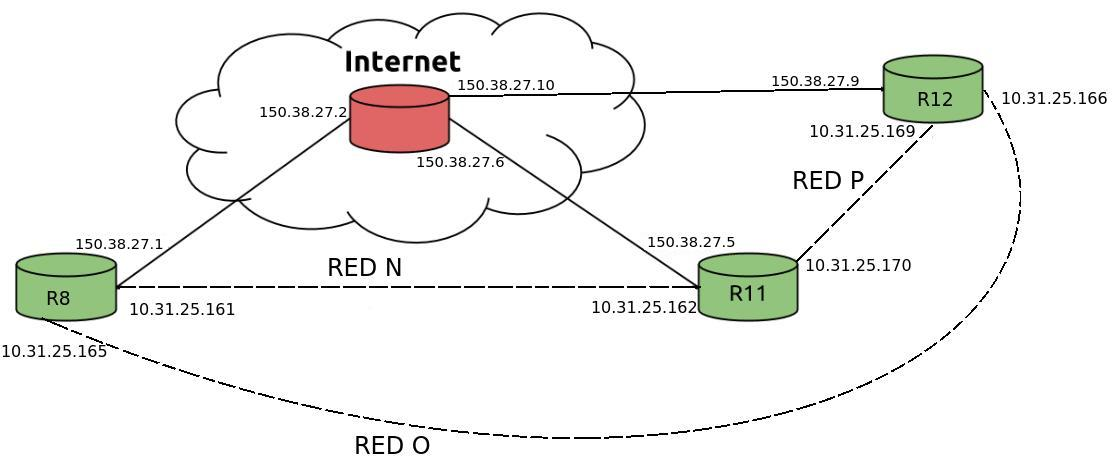
\includegraphics[width=\textwidth]{gre.jpeg} 
\label{gre}
\caption{Esquema de Tunel GRE}
\end{figure}


\section{VRRP}
\subsection{Configuración de los Routers}
\paragraph{R4}
{\small
\begin{verbatim}
track 1 interface Ethernet0/0 ip routing
track 2 interface Ethernet0/1 ip routing

interface Ethernet0/0
 description Conexion LAN Red A
 ip address 201.158.15.3 255.255.255.128
 full-duplex
 vrrp 10 ip 201.158.15.7
 vrrp 10 timers advertise 15
 vrrp 10 timers learn
 vrrp 10 priority 110
 vrrp 10 track 1 decrement 20
 vrrp 10 track 2 decrement 20

interface Ethernet0/1
 description Conexion LAN Red D
 ip address 20.64.73.2 255.255.255.0
 full-duplex
 vrrp 11 ip 20.64.73.5
 vrrp 11 timers advertise 15
 vrrp 11 timers learn
 vrrp 11 priority 110
 vrrp 11 track 1 decrement 20
 vrrp 11 track 2 decrement 20
\end{verbatim}
}

\paragraph{R5}
{\small
\begin{verbatim}
track 1 interface Ethernet0/0 ip routing
track 2 interface Ethernet0/1 ip routing

interface Ethernet0/0
 description Conexion LAN Red A
 ip address 201.158.15.4 255.255.255.128
 full-duplex
 vrrp 10 ip 201.158.15.7
 vrrp 10 timers advertise 15
 vrrp 10 timers learn
 vrrp 10 priority 100
 vrrp 10 track 1 decrement 20
 vrrp 10 track 2 decrement 20

interface Ethernet0/1
 description Conexion LAN Red D
 ip address 20.64.73.1 255.255.255.0
 full-duplex
 vrrp 11 ip 20.64.73.5
 vrrp 11 timers advertise 15
 vrrp 11 timers learn
 vrrp 11 priority 100
 vrrp 11 track 1 decrement 20
 vrrp 11 track 2 decrement 20
\end{verbatim}
}


\section{DNS}

\subsubsection{Niveles de servidores DNS}

Para la realización del trabajo práctico es necesario implementar el servicio de DNS, dividido en las distintas sedes de la topología, para así poder traducir nombres a direcciones IP (para permitir la comunicación) o viceversa (por ejemplo, para el uso de traceroute). \\ 

Se dispone de tres servidores DNS, uno de primer nivel (DNS root) y dos de segundo nivel (llamados DNS 1 y DNS 2). El DNS 1 tiene autoridad sobre la sede La Falda y el DNS 2 sobre el resto de la red (sedes Calamuchita y Córdoba Capital). Los hosts que deseen traducir un nombre o una IP deben consultar al servidor DNS de segundo nivel que corresponda a su zona. En caso de que dicho servidor pueda realizar la traducción, transmite la consulta hacia el DNS Root. \\

\subsubsection{Nombres de dominio de redes}


\begin{tabular}{|c|c|c|c|c|}
	\hline
	Subnet & Nombre & Nombre de dominio &  Sede\\
	\hline
	A & Águila & aguila.capital.cordoba.dc.fi.uba.ar &  Capital \\
	\hline
	B & Buitre & buitre.capital.cordoba.dc.fi.uba.ar & Capital \\
	\hline
	C & Cuervo & cuervo.capital.cordoba.dc.fi.uba.ar & Capital \\
	\hline
	D & Dodo & dodo.capital.cordoba.dc.fi.uba.ar & Capital \\
	\hline
	E & Espátula & espatula.lafalda.cordoba.dc.fi.uba.ar & La Falda \\
	\hline
	F & Faisán & faisan.lafalda.cordoba.dc.fi.uba.ar & La Falda \\
	\hline
	G & Golondrina & golondrina.calamuchita.cordoba.dc.fi.uba.ar & Calamuchita \\
	\hline
	H & Hornero & hornero.calamuchita.cordoba.dc.fi.uba.ar & Calamuchita \\
	\hline
	I1 & Ibis 1 & ibis1.calamuchita.cordoba.dc.fi.uba.ar & Calamuchita \\
	\hline
	I2 & Ibis 2 & ibis2.calamuchita.cordoba.dc.fi.uba.ar &  Calamuchita \\ 
	\hline
	I3 & Ibis 3 & ibis3.calamuchita.cordoba.dc.fi.uba.ar &  Calamuchita \\
	\hline
	I4 & Ibis 4 & ibis4.calamuchita.cordoba.dc.fi.uba.ar & Calamuchita \\
	\hline
	I5 & Ibis 5 & ibis5.calamuchita.cordoba.dc.fi.uba.ar &  Calamuchita \\	
	\hline
	I6 & Ibis 6 & ibis6.calamuchita.cordoba.dc.fi.uba.ar &  Calamuchita \\
	\hline
	I7 & Ibis 7 & ibis7.calamuchita.cordoba.dc.fi.uba.ar &  Calamuchita \\
	\hline
	I8 & Ibis 8 & ibis8.calamuchita.cordoba.dc.fi.uba.ar &  Calamuchita \\
	\hline
	I9 & Ibis 9 & ibis9.calamuchita.cordoba.dc.fi.uba.ar &  Calamuchita \\
	\hline
	I10 & Ibis 10 & ibis10.calamuchita.cordoba.dc.fi.uba.ar &  Calamuchita \\
	\hline
	J & Jilguero & jilguero.lafalda.cordoba.dc.fi.uba.ar &  La Falda \\
	\hline
	K & Kiwi & kiwi.lafalda.cordoba.dc.fi.uba.ar & La Falda \\
	\hline
	L & Lechuza & lechuza.calamuchita.cordoba.dc.fi.uba.ar & Calamuchita \\
	\hline
	M1 & Mero 1 & mero1.calamuchita.cordoba.dc.fi.uba.ar & Calamuchita \\
	\hline
	M2 & Mero 2 & mero2.calamuchita.cordoba.dc.fi.uba.ar & Calamuchita \\
	\hline
	N privada & Negrón & negron.calamuchita.cordoba.dc.fi.uba.ar & Calamuchita \\
	\hline
	O privada & Ortega & ortega.calamuchita.cordoba.dc.fi.uba.ar & Calamuchita \\
	\hline
	P privada & Paloma & paloma.calamuchita.cordoba.dc.fi.uba.ar & Calamuchita \\
	\hline
	Q1 Publica & Quebrantahuesos 1 & quebrantahuesos1.calamuchita.cordoba.dc... &  Calamuchita \\
	\hline
	Q2 Publica & Quebrantahuesos 2 & quebrantahuesos2.calamuchita.cordoba.dc... & Calamuchita \\
	\hline
	Q3 Publica & Quebrantahuesos 3 & quebrantahuesos3.calamuchita.cordoba.dc... &  Calamuchita \\
	\hline
\end{tabular}




\section{OpenVPN}
Para realizar el trabajo práctico fue necesario la creación de 9 VPNs\footnote{Los 9 dispositivos son: Host A, Host B, Host C, DNS1, DNS2, DNS Root, Telserver, WebServer y FTPServer}, para poder conectar los distintos dispositivos físicos a la red simulada en GNS3. Notamos que, aunque sólo 5 de éstos servicios estarían en simultáneo utilizándose (los DNSs, alguno de los 3 hosts, y alguno de los servicios), es necesario tener todo configurado para poder cambiar a otro dispositivo (siendo mucho más fácil configurando distintas VPNs).

REVISAR: el telserver no tenía dos taps? serían 10 entonces....

\subsection{Servidores}
Dentro de la PC que corre la topología en GNS3 se tiene a los 9 VPNs ejecutándose en paralelo (en 9 puertos diferentes). Para cada uno de estos se configura la interfaz tap correspondiente. 

\subsection{Clientes}
Para cada uno de los clientes se crearon los scripts correspondientes para poder conectar al servidor, el cual cuenta con la dirección IP con la que deberá conectarse, el puerto al que debe conectarse (para conectarse a una determinada interfaz tap del servidor), el certificado, máscara de subred, y otros parámetros. Además, es necesario configurar la tabla de ruteo para tal cliente (como ya fue determinada en la sección de Tablas de Ruteo Estático).

\section{Scripts de configuración}
Para realizar la simulación de la topología, y poder utilizar los distintos dispositivos físicos, comunicados por las interfaces taps (como ya fue explicado en secciones anteriores), se crearon scripts para automatizar la ejecución de los mismos. A continuación se detallan los distintos tipos de scripts:
\begin{itemize}
	\item \textbf{Servicios.sh}: Permite levantar los servicios de telnet, apache o ftp.
	\item \textbf{pings.sh}: Realiza una secuencia de pings a dispositivos a lo largo de toda la topología. Lo utilizamos para corroborar la
		 correcta conexión entre los dispositivos físicos con el servidor que ejecuta al GNS3, así como asegurar la correcta configuración
		 del ruteo estático.
	\item \textbf{levantarHostA.sh}: Se configura la interfaz tap correspondiente; se configura el ruteo estático para tal host; se copia el 
		archivo \textbf{resol.conf} al directorio local para dejar configurado el DNS de nuestra topología (para el caso del host A, el DNS2).
		Para los Hosts B y C se tienen análogos archivos de configuración (con los parámetros correspondientes).
	\item \textbf{levantarWebserver.sh}: similar al caso anterior, pero en este caso además copia los archivos de configuración necesarios al
		directorio local correspondiente. Tanto para el FTPserver como para el TelServer se cuenta con sus semejantes archivos de 
		configuración.
	\item \textbf{finalizarVPNs.sh}: cierra todas las conexiones taps utilizadas (del 0 al 9) en el dispositivo local.
\end{itemize}

\newpage
\section{Anexos}
\subsection{Topología de la Red}
\begin{figure}[h!]
\centering
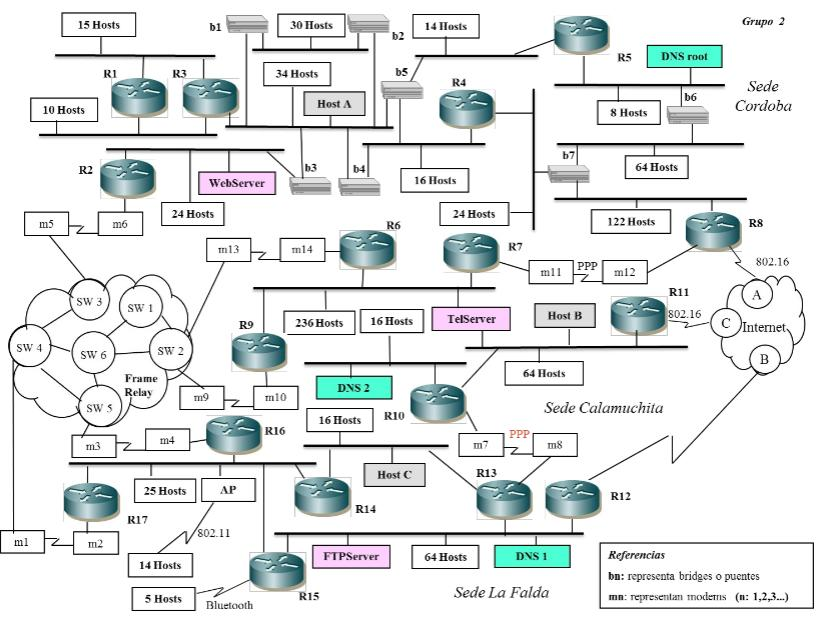
\includegraphics[width=\textwidth]{topologia.jpeg}
\label{topologia}
\caption{Topología de la Red}
\end{figure}

\newpage
\subsection{Topología de la Red, con división de Subredes}
\begin{figure}[h!]
\centering
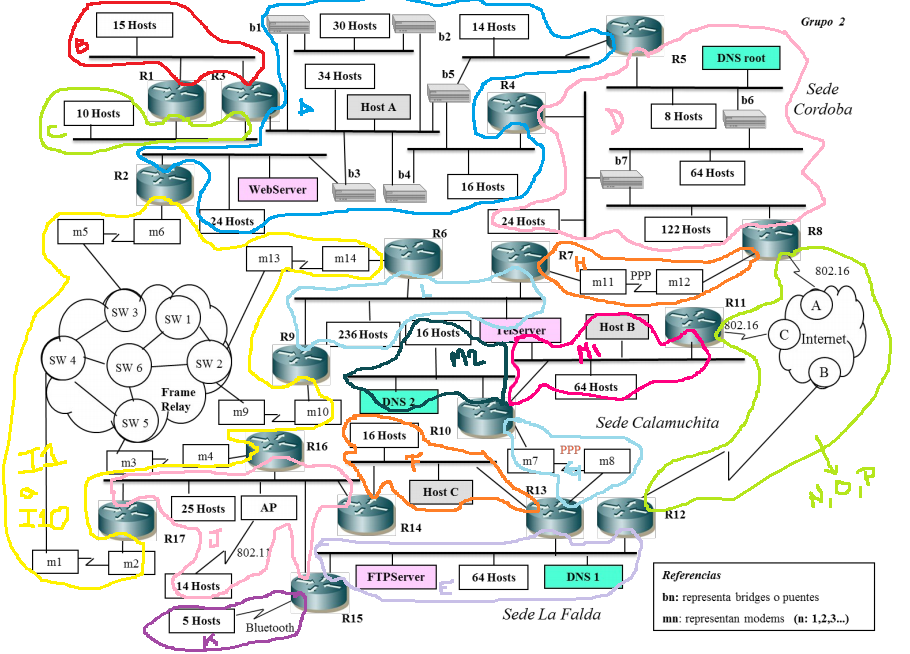
\includegraphics[width=\textwidth]{DivisionRedes.png}
\label{topologia}
\caption{Topología de la Red}
\end{figure}

\newpage
\subsection{Diagrama de Capa 3, con direcciones IP}
\begin{figure}[h!]
\centering
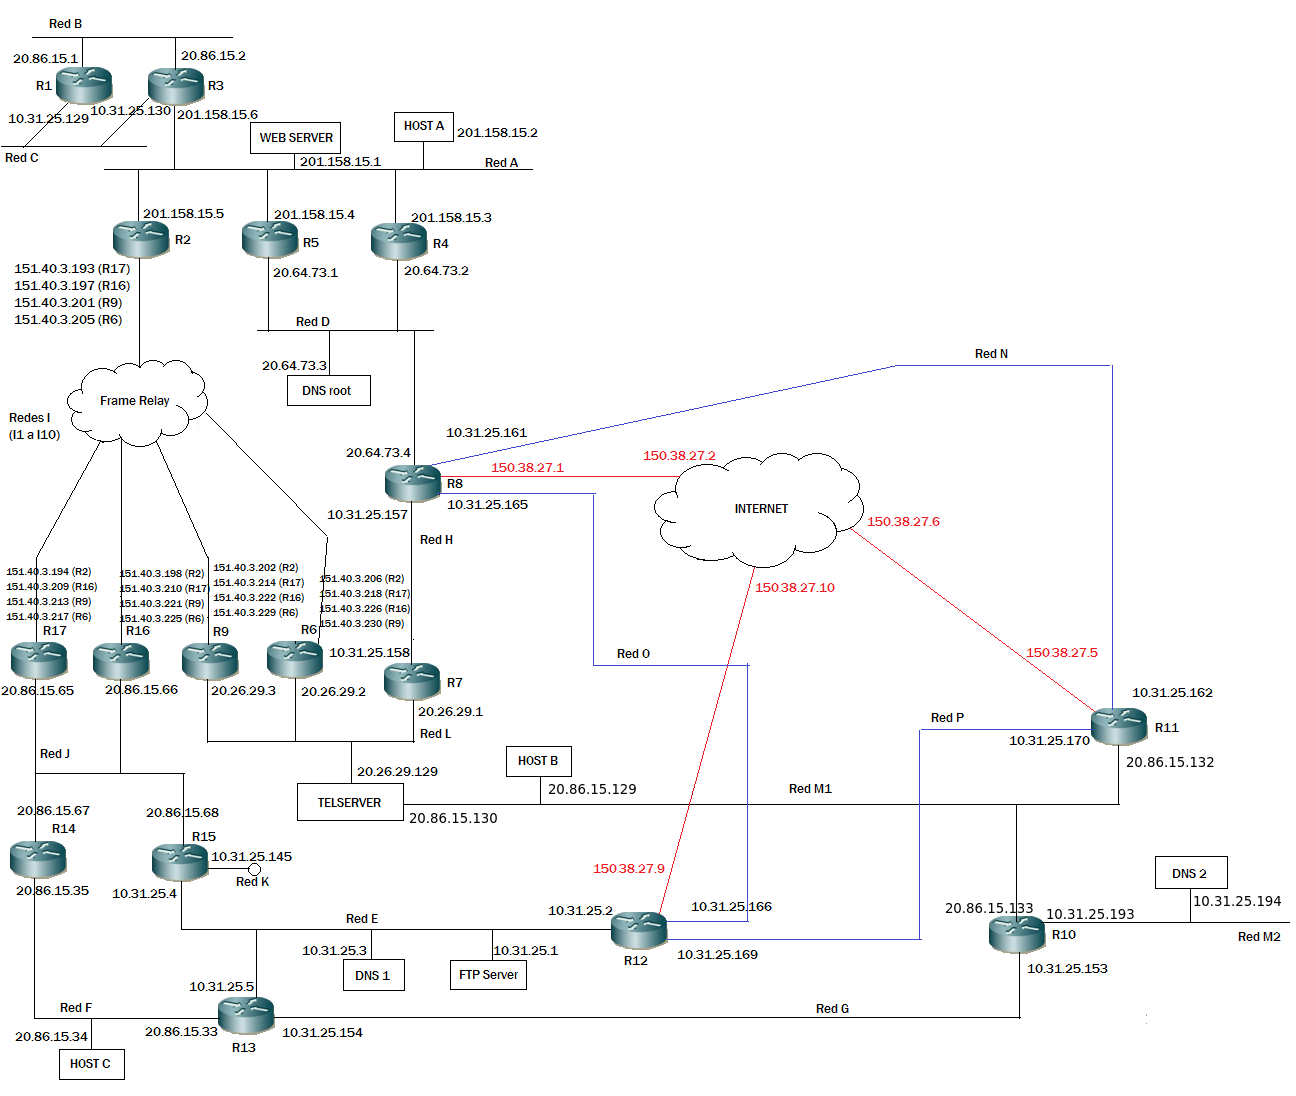
\includegraphics[width=\textwidth]{DiagramaCapa3conIPs.png}
\label{topologia}
\caption{Topología de la Red}
\end{figure}
\end{document}
